%%%%%%%%%%%%%%%%%%%%%%%%%%%%%%%%%%%%%%%%%%  不使用 authblk 包制作标题  %%%%%%%%%%%%%%%%%%%%%%%%%%%%%%%%%%%%%%%%%%%%%%
%-------------------------------PPT Title-------------------------------------
\title{15-\rm{LDA/GGA}+$U$与自相互作用校正}
%-----------------------------------------------------------------------------
%----------------------------Author & Date------------------------------------

%\author[\textrm{Jun\_Jiang}]{姜\;\;骏\inst{}} %[]{} (optional, use only with lots of authors)
%% - Give the names in the same order as the appear in the paper.
%% - Use the \inst{?} command only if the authors have different
%%   affiliation.
%\institute[BCC]{\inst{}%
\institute[Gain~Strong]{\inst{}%
%\vskip -20pt 北京市计算中心}
\vskip -20pt {\large 格致斯创~科技}}
\date[\today] % (optional, should be abbreviation of conference name)
{%	{\fontsize{6.2pt}{4.2pt}\selectfont{\textcolor{blue}{E-mail:~}\url{jiangjun@bcc.ac.cn}}}
\vskip 45 pt {\fontsize{8.2pt}{6.2pt}\selectfont{%清华大学\;\;物理系% 报告地点
	\vskip 5 pt \textrm{2023.07.01}}}
}

%% - Either use conference name or its abbreviation
%% - Not really information to the audience, more for people (including
%%   yourself) who are reading the slides onlin%%   yourself) who are reading the slides onlin%%   yourself) who are reading the slides onlineee
%%%%%%%%%%%%%%%%%%%%%%%%%%%%%%%%%%%%%%%%%%%%%%%%%%%%%%%%%%%%%%%%%%%%%%%%%%%%%%%%%%%%%%%%%%%%%%%%%%%%%%%%%%%%%%%%%%%%%

\subject{}
% This is only inserted into the PDF information catalog. Can be left
% out.
%\maketitle
\frame
{
%	\frametitle{\fontsize{9.5pt}{5.2pt}\selectfont{\textcolor{orange}{“高通量并发式材料计算算法与软件”年度检查}}}
\titlepage
}
%-----------------------------------------------------------------------------

%------------------------------------------------------------------------------列出全文 outline ---------------------------------------------------------------------------------
\section*{}
\frame[allowframebreaks]
{
  \frametitle{Outline}
%  \frametitle{\textcolor{mycolor}{\secname}}
  \tableofcontents%[current,currentsection,currentsubsection]
}
%%在每个section之前列出全部Outline
%%类似的在每个subsection之前列出全部Outline是\AtBeginSubsection[]
%\AtBeginSection[]
%{
%  \frame<handout:0>%[allowframebreaks]
%  {
%    \frametitle{Outline}
%%全部Outline中,本部分加亮
%    \tableofcontents[current,currentsection]
%  }
%}

%-----------------------------------------------PPT main Body------------------------------------------------------------------------------------
\small
%\section{\rm{VASP~}软件中\rm{PAW~}计算的实现}
%\frame
%
%	\frametitle{\textrm{VASP}计算的特色}
%	相比于与普通的第一原理计算软件,\textrm{VASP}很好地平衡了计算效率和精度的问题,总的来说,\textrm{VASP}主要通过这几个特色保证了计算的高效能
%	\begin{itemize}
%	     \item 迭代与优化算法的多样性\\
%		     本质上电荷密度迭代 \textrm{\&\&} 体系总能量优化是相同的优化问题,采用了类似的算法\upcite{CMS6-15_1996,PRB54-11169_1996}:\\
%			\textcolor{blue}{\textrm{Pseudo-Newton、Conjugate-Gradient、Broyden~mix、damping-factor、RMM-DIIS}}
%	     \item 尽可能采用局域基(原子轨道基)函数:~\\
%		     \textcolor{blue}{\textrm{LREAL}}=\textcolor{red}{\textrm{.TRUE.}}\\
%			优化的投影函数也尽可能在实空间表示
%	     \item \textrm{PAW}原子数据集:\textcolor{blue}{优异的赝势}\upcite{PRB59-1758_1999}
%	\end{itemize}
%}
\section{\rm{LDA+}$U$与自相互作用校正}
\subsection{\rm{LDA}与精确交换-相关泛函}
\frame
{
	\frametitle{\textrm{L(S)DA}方法的不足}
	\begin{itemize}
		\item 一般对只含$s$、$p$价电子体系,基于\textrm{DFT(L(S)DA/GGA)\,}的结构、能带计算都能给出令人满意的结果
	\end{itemize}
\begin{figure}[h!]
\centering
\vspace*{-0.25in}
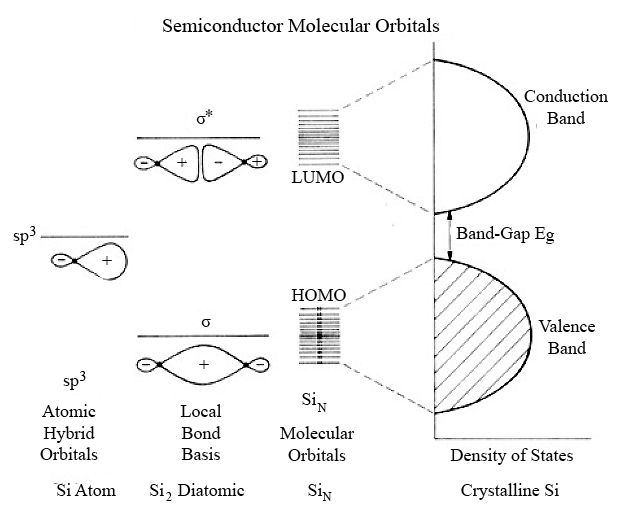
\includegraphics[height=2.25in,width=3.1in,viewport=0 0 630 560,clip]{Figures/Combination-of-atomic-orbital-to-molecular-orbital-and-to-band-gap-of-silicon-molecule.png}
\caption{\tiny \textrm{Combination of atomic orbital to molecular orbital and to band gap of silicon molecule.}}%(与文献\cite{EPJB33-47_2003}图1对比)
\label{LDA_U-1}
\end{figure}
}

\frame
{
	\frametitle{\textrm{L(S)DA}方法的不足}
	\begin{itemize}
		\item 但是对价电子包含$d$和$f$局域电子体系,特别是过渡金属氧化物或氮化物(\textcolor{orange}{如\textrm{Mott}\,绝缘体}),在“金属/绝缘体”的定性判断上,\textrm{L(S)DA/GGA}\,计算结果常常出错
	\end{itemize}
\begin{figure}[h!]
\centering
\vspace*{-0.20in}
%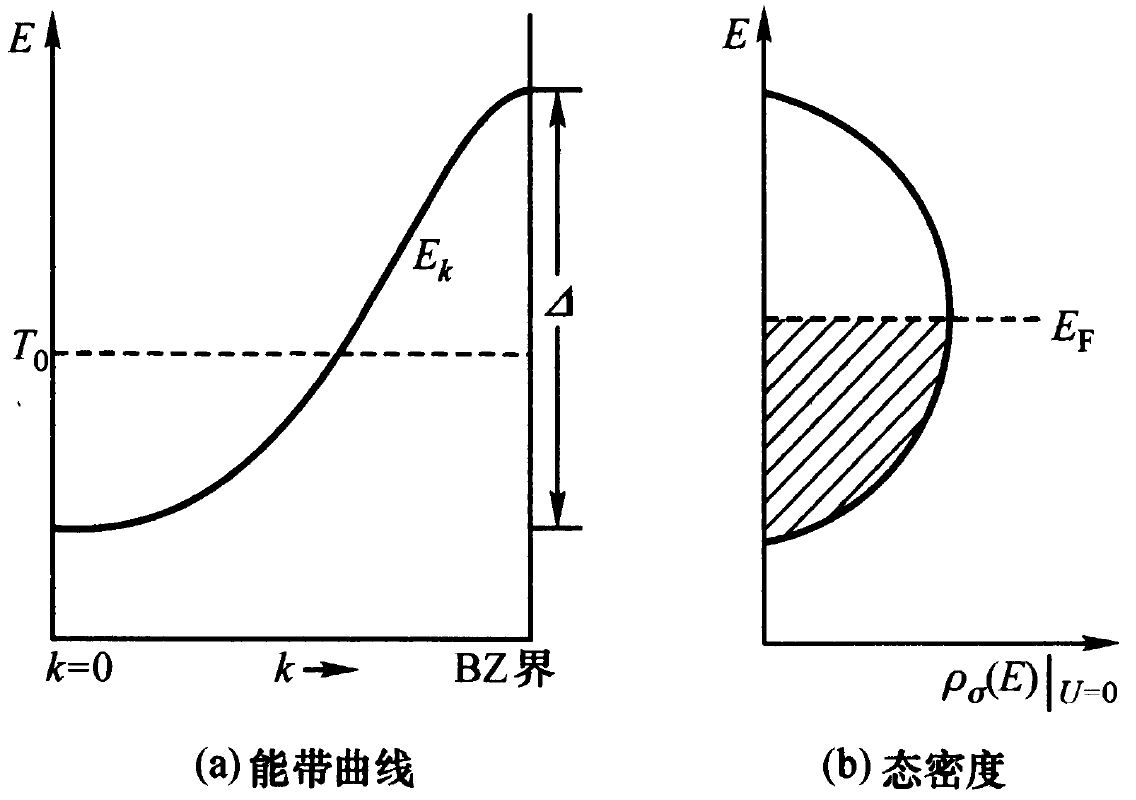
\includegraphics[height=2.05in,width=3.2in,viewport=0 0 1200 880,clip]{Figures/LDA_U-3.png}
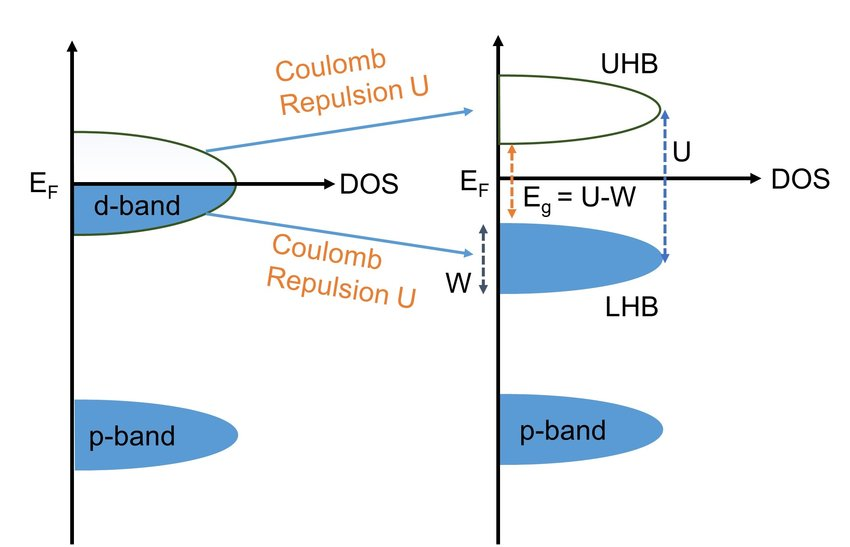
\includegraphics[height=2.05in,width=3.1in,viewport=0 0 205 140,clip]{Figures/Band-diagram-of-Mott-Hubbard-Insulator.jpg}
\caption{\tiny \textrm{The schematic band structure of Mott-Hubbard-Insulator:~independent electron (left) correlation electron (right).}}%(与文献\cite{EPJB33-47_2003}图1对比)
\label{LDA_U-3}
\end{figure}
}

\frame
{
	\frametitle{\textrm{Mott-Hubbard Insulator}}
\begin{figure}[h!]
\centering
\vspace*{-0.20in}
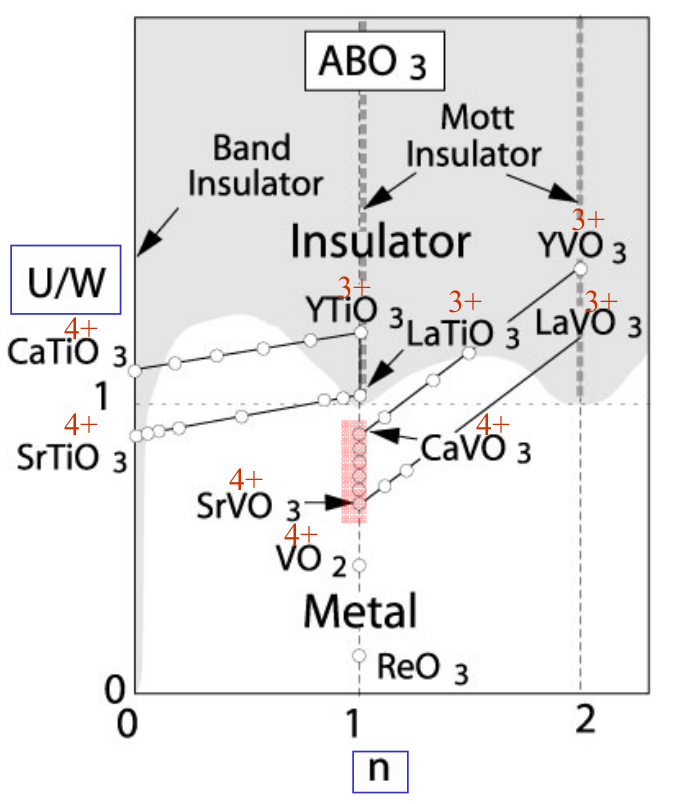
\includegraphics[height=2.70in,width=2.2in,viewport=0 0 660 840,clip]{Figures/Band-Mott_Hubard-Insulator.jpeg}
\caption{\tiny \textrm{The schematic bandwidth vs. filling-controlled in Mott-Hubbard system of Perovskite structure.}}%(与文献\cite{EPJB33-47_2003}图1对比)
\label{Bandwidth-Mott_Hubard-Insulator}
\end{figure}
}

\frame
{
	\frametitle{\textrm{Mott-Hubbard vs. charge transfer insulator.}}
\begin{figure}[h!]
\centering
\vspace*{-0.10in}
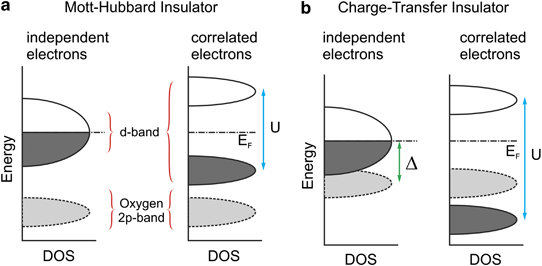
\includegraphics[height=2.30in,width=4.0in,viewport=0 0 320 170,clip]{Figures/Schematic-energy-band-diagrams-of-a-Mott-Hubbard-insulator-and-a-charge-transfer-insulator-independent_left-correlation_right.jpg}
\caption{\tiny \textrm{Schematic energy band diagrams of a Mott-Hubbard insulator (a) and a charge transfer insulator (b): independent electrons(left)  and correlation electrons (right).}}%(与文献\cite{EPJB33-47_2003}图1对比)
\label{Band-Mott_Hubard_vs_charge-Insulator}
\end{figure}
}

\frame
{
	\frametitle{密度\textrm{vs.}粒子与泛函表示}
\begin{figure}[h!]
\vskip -10pt
\centering
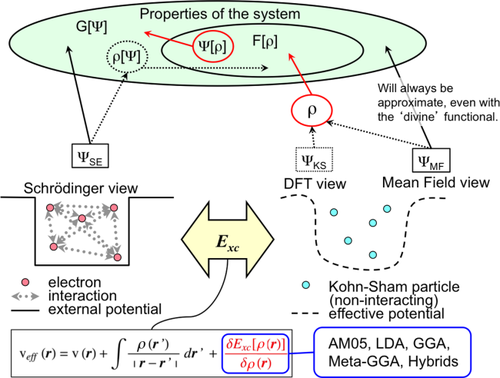
\includegraphics[height=2.65in,width=3.8in,viewport=0 0 362 275,clip]{Figures/DFT-particle-density.png}
\caption{\fontsize{6.0pt}{4.5pt}\selectfont{\textrm{Properties of a quantum mechanical system can be calculated by solving the SE (left). A more tractable, formally equivalent way is to solve the DFT KS equations (right).}}}%(与文献\cite{EPJB33-47_2003}图1对比)
\label{Schrodinger-equation-vs-Kohn-Sham-equation}
\end{figure}
}

\frame
{
	\frametitle{密度\textrm{vs.}粒子与泛函表示}
\begin{itemize}
\setlength{\itemsep}{12pt}
	\item 精确密度泛函具有当电子数在整数值前后改变的时候,体系能量的改变是不连续的属性,单电子能量的不连续对能带的带隙有很大贡献
	 \item\textrm{LD(S)A~}近似中体系能量是电子数的连续函数,不具备体系能量随电子数变化不连续的特征。\textrm{LDA/GGA~}方法在描述含有$d$/$f$电子的过渡金属和稀土元素化合物体系时常常失效。
	\item \textrm{LDA}/\textrm{GGA~}得到的体系总能量和实验结果符合较好,但轨道能量(即$\varepsilon_i=\partial E/\partial n_i$),不符合\textrm{Koopmans~}定理,与实验或者严格计算得到的轨道能量差别很大%一个典型的例子就是对H原子的计算结果,LDA计算的轨道能级为$-$0.27\,a.u.(实验结果为$-$0.5\,a.u.),总能量($-$0.488\,a.u.)则非常接近$-$0.5\,a.u.\upcite{PRB37-9919_1988}。
%	\item \textrm{Anisimov~}提出通过对\textrm{LDA~}势加入轨道校正克服不足(称为\textrm{LDA+$U$}方法)\upcite{PRB44-943_1991,PRB48-16929_1993}%LDA+U方法与Andersen掺杂模型\upcite{PR124-41_1961}思想类似,
\end{itemize}
}

\frame
{
	\frametitle{精确交换-相关泛函的特征}
	\textrm{Perdew}指出\upcite{PRL49-1691_1982},尽管交换-相关泛函的精确形式不知,但总能量泛函对电子数的依赖$E(N)$应该具有折线形式
\begin{figure}[h!]
\centering
\vspace*{-0.1in}
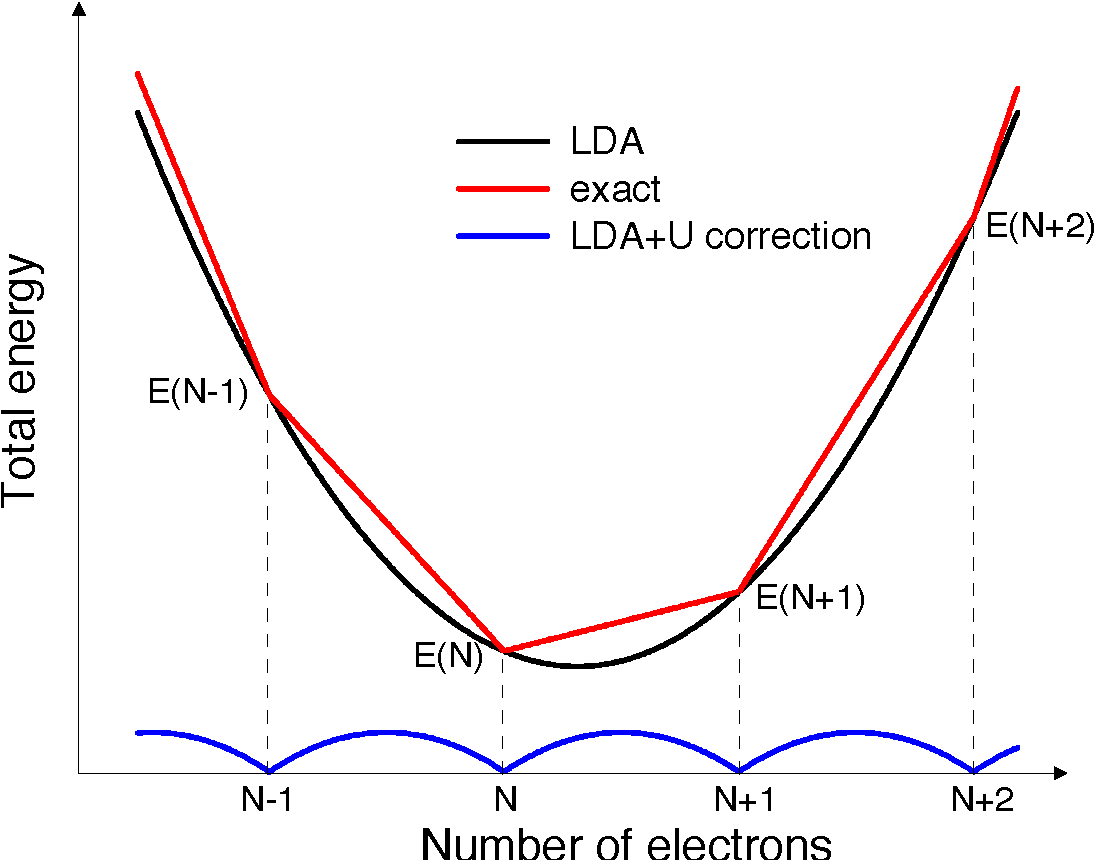
\includegraphics[height=2.2in,width=3.1in,viewport=0 0 1200 890,clip]{Figures/Koopmans-condition_LDA-U.png}
\caption{\tiny \textrm{The dependence of the total energy on the number of electron is a series of straight-line segments.}}%(与文献\cite{EPJB33-47_2003}图1对比)
\label{exact-DFT}
\end{figure}
}

\frame
{
	\frametitle{\textrm{L(S)DA}与精确交换-相关泛函}
	\begin{itemize}
		\item $E(N)$\textcolor{blue}{曲线本身连续}
	\begin{displaymath}
		\dfrac{\partial E}{\partial N}=\left\{
		\begin{aligned}
			E(M)-E(M-1)\qquad M-1<N<M\\
			E(M+1)-E(M)\qquad M<N<M+1 
		\end{aligned}\right.
	\end{displaymath}
		\item 导数$\partial E/\partial N$\textcolor{red}{在跨越整数电子时不连续}

	类似地,精确的单电子势$V(\vec r)=\dfrac{\delta E}{\delta n(\vec r)}$\\
	\textcolor{blue}{在电子数出现整数变化时同样存在不连续的跳跃}
		\item \textrm{L(S)DA}近似下,能量$E$对电子数$N$曲线及其导数\textcolor{red}{\underline{都是连续的}}
	
			\vspace{10pt}
	\textcolor{blue}{\textrm{L(S)DA}近似对\textrm{Mott}绝缘体计算的失效}:\\
	\textcolor{red}{单电子势函数不满足电子数整数变化时跳跃的不连续要求}
	\end{itemize}
}

\frame
{
	\frametitle{平均场模型:~\textrm{L(S)DA}与\textrm{HF}的关系}
	\begin{itemize}
		\item \textrm{DFT}以密度$\rho(\vec r)$作为基本变量\\
		\textrm{LDA}的势函数仅是电荷密度的函数\\
%		电荷密度由总电荷(或平均轨道占据数)确定,
		\textcolor{red}{包含了电子自相互作用}
		
		\item \textrm{HF}的基本变量是波函数$\Psi(\vec r)$\\
			存在交换作用$\mathrm{J}$\\
		\textcolor{red}{扣除了自旋同向电子的自相互作用}
		\item \textrm{LDA}与\textrm{HF}的相似性:\\
			对于含有$d$价电子体系,如果$d$轨道电子占据数为$n_{m,\sigma}$\\
			\textcolor{blue}{当电子对轨道平均占据}
		$$n_0=\dfrac{\sum\limits_{m,\sigma}n_{m,\sigma}}{10}$$
		\textcolor{blue}{\textrm{HF}计算与基于\textrm{LDA}的\textrm{DFT}计算将给出一致的结果}
	\end{itemize}
}

%\subsection{自旋极化与金属磁矩}
%\frame
%{
%	\frametitle{自旋极化与磁矩}
%	考虑自旋极化(\textrm{LSDA})的体系总能量泛函
%	\begin{displaymath}
%		\begin{aligned}
%			E^{\mathrm{LSDA}}=&E^{\mathrm{LDA}}\{n(\vec r)\}+E_{xc}\{n_{\uparrow}(\vec r),n_{\downarrow}(\vec r)\}\\
%			-&E_{xc}^{\mathrm{LDA}}\{n(\vec r)\}
%		\end{aligned}
%	\end{displaymath}
%	$E^\mathrm{{LDA}}$是非磁性态的能量,是电荷密度分布分布$\{n(\vec r)\}$的函数,$E_{xc}$是与自旋电荷密度分布有关的交换-相关泛函\\
%	由于交换引起的势函数移动可以用体系磁化强度$m(\vec r)$表示
%	\begin{displaymath}
%		V_{\uparrow}-V_{\downarrow}=\frac{\delta E^{\mathrm{LSDA}}}{\delta n_{\uparrow}(\vec r)}-\frac{\delta E^{\mathrm{LSDA}}}{\delta n_{\downarrow}(\vec r)}=f(\vec r)m(\vec r)
%	\end{displaymath}
%	根据\textrm{Stoner}模型,当体系处于弱磁化态,交换效应引起的能带裂分近似与波矢$\vec k$无关
%	\begin{displaymath}
%		\langle\psi_j^{\vec k}|f(\vec r)m(\vec r)|\psi_j^{\vec k}\rangle\sim-mI
%	\end{displaymath}
%}
%
%\frame
%{
%	\frametitle{交换作用与自发磁化}
%\begin{itemize}
%	\item \textrm{Slater}考虑了自旋相同电子间的交换作用,\textcolor{blue}{相当于体系内部存在一个沿正方向的内磁场},引起能带劈裂$\Delta$\upcite{Dai_Qian}
%\begin{figure}[h!]
%\centering
%\vspace*{-0.05in}
%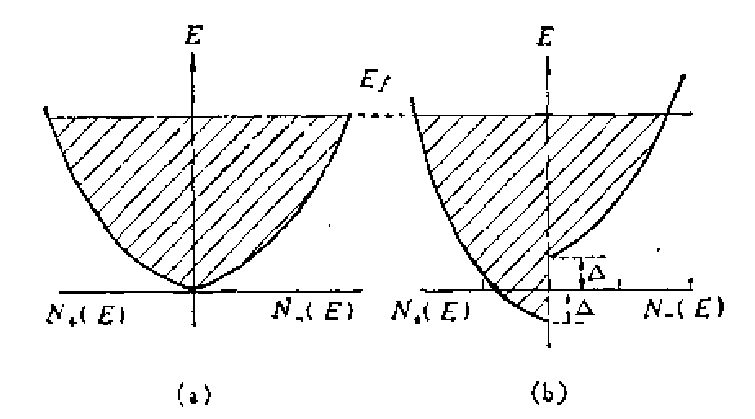
\includegraphics[height=0.9in,width=1.8in,viewport=0 0 800 380,clip]{Figures/Mag_Metal-exchange.png}
%\caption{\tiny \textrm{The exchange and the splitted band.}}%(与文献\cite{EPJB33-47_2003}图1对比)
%\label{Mag_Metal-exchange}
%\end{figure}
%	\item $\Delta$的大小与电子间交换作用直接关联
%	\item 考虑交换作用后,每个原子上净的自旋电子数目不再相等,有可能发生自发磁化
%	\item 自发磁化态是铁磁(Ferromagnet)还是反铁磁(Anti-Ferromagnet),则由体系交换作用的特点决定
%\end{itemize}
%}
%
%\frame
%{
%	\frametitle{\textrm{Stoner}模型}
%	\begin{itemize}
%		\item \textrm{Stoner}将金属的磁性考虑为晶格中巡游的$3d$、$4s$\,电子贡献,其相互作用为$I$,\textrm{Fermi}面附近的\textrm{DOS}为$N(E_{\mathrm F})$
%\begin{figure}[h!]
%\centering
%\vspace*{-0.05in}
%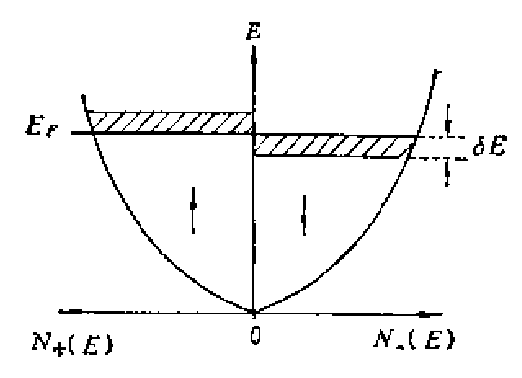
\includegraphics[height=1.0in,width=1.8in,viewport=0 0 800 380,clip]{Figures/Mag_Metal-T0.png}
%\caption{\tiny \textrm{The Stoner model.}}%(与文献\cite{EPJB33-47_2003}图1对比)
%\label{Mag_Metal-T0}
%\end{figure}
%		\item 体系的磁性由转变由\textrm{Fermi}面附近能量变化确定
%			\begin{displaymath}
%				\Delta E=N(E_{\mathrm F})\big[1-IN(E_{\mathrm F})\big](\delta E)^2
%			\end{displaymath}
%	\end{itemize}
%}
%
%\frame
%{
%	\frametitle{\textrm{Stoner}模型}
%	\begin{itemize}
%		\item \textrm{Stoner}模型中参数$I$\,主要反应$3d$电子的紧束缚特征,与晶体结构关系不大
%		\item \textrm{Stoner}用于孤立原子体系,参数$I$描述自旋电子的裂分,要求:
%			\begin{enumerate}
%				\item \textcolor{blue}{对\textrm{LSDA}描述的单行列式态,参数$I$可以精确描述原子态的裂分}
%				\item \textcolor{blue}{\textrm{LSDA}中应用\textrm{Stoner}模型,参数$I$\,与\textrm{Hund}规则的交换参数$J$一致}
%			\end{enumerate}
%		\item 参数$U$、$I$(或$J$~)的大小\\
%			\begin{enumerate}
%				\item \textcolor{red}{\textrm{Hund}规则的交换参数$J$的数量级:~ \textrm{1eV}
%				\item \textrm{Hubbard}参数$U$的数量级:~\textrm{10eV}}
%			\end{enumerate}
%	\end{itemize}
%}

\subsection{$U$值的物理含义}
\frame
{
	\frametitle{从晶体场的角度看待能带列分}
\begin{figure}[h!]
\centering
\vspace*{-0.22in}
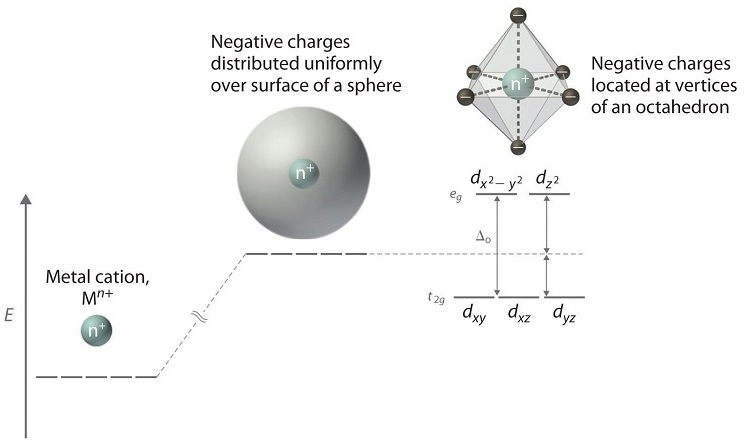
\includegraphics[height=1.45in,width=2.62in,viewport=0 0 585 350,clip]{Figures/Crystal-Field-Theory.jpg}
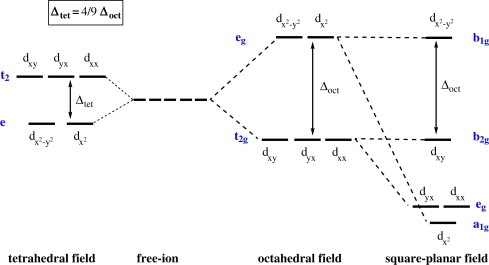
\includegraphics[height=1.25in,width=3.32in,viewport=0 0 315 170,clip]{Figures/Crystal-Field-Theory_energy.jpg}
\caption{\tiny \textrm{The schematic illustration of Crystal Field Theory (CFT) for the splitting of \textit{d}-orbital.}}%(与文献\cite{EPJB33-47_2003}图1对比)
\label{CFT_d-splitting}
\end{figure}
}
 
\frame
{
\frametitle{$U$值的物理含义}
\textrm{Hubbard}模型(\textrm{Anderson晶格模型}):\\含有$n$个$d$、$f$\,电子的强关联体系中,关联电子间最重要的相互作用是原子内在位(\textrm{on-site})相互作用$U$
\begin{figure}[h!]
\centering
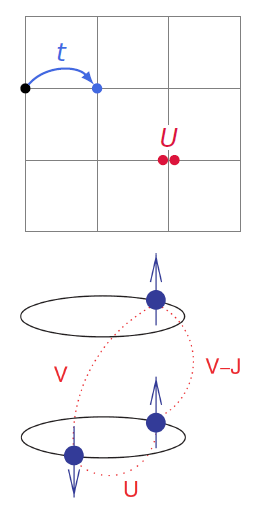
\includegraphics[height=1.25in,width=0.92in,viewport=1 1 240 375,clip]{Figures/LDA_U-1.png}
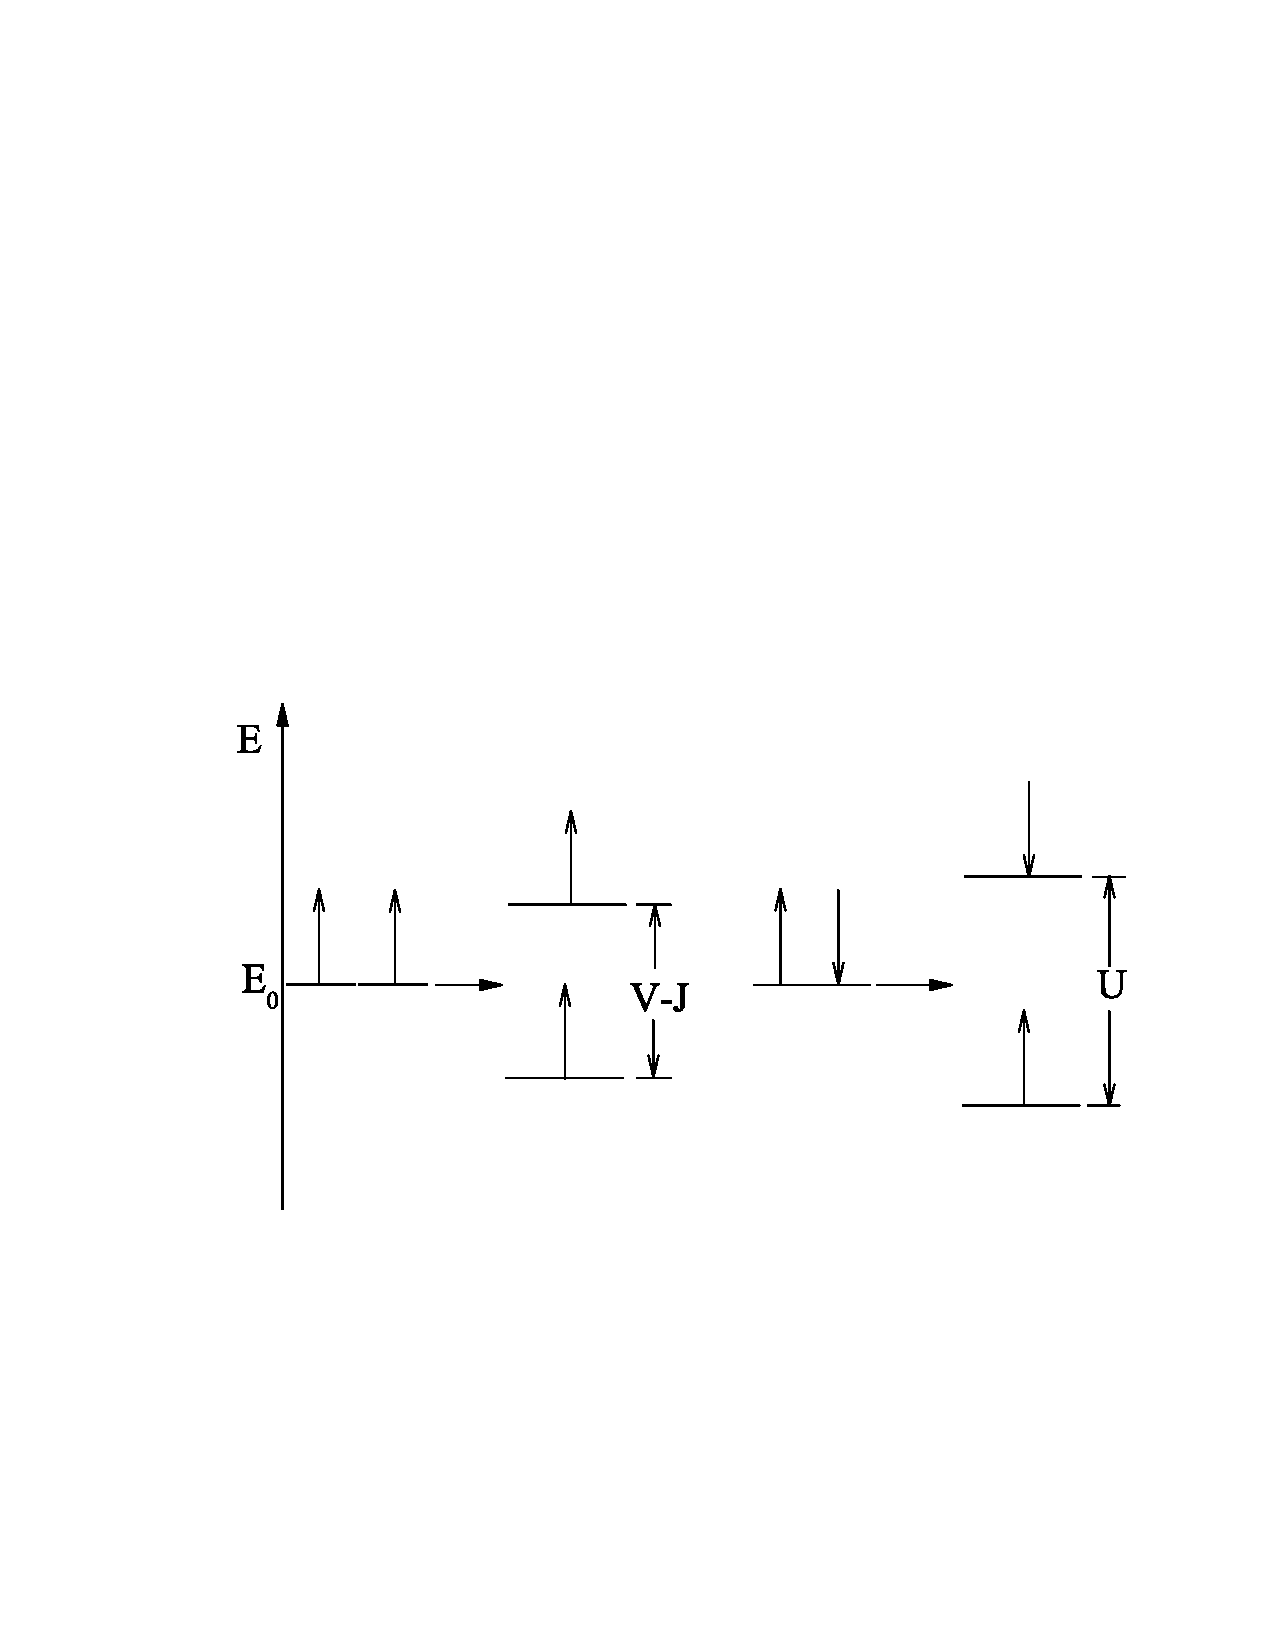
\includegraphics[height=1.25in,width=2.32in,viewport=110 210 545 455,clip]{Figures/LDA_U.pdf}
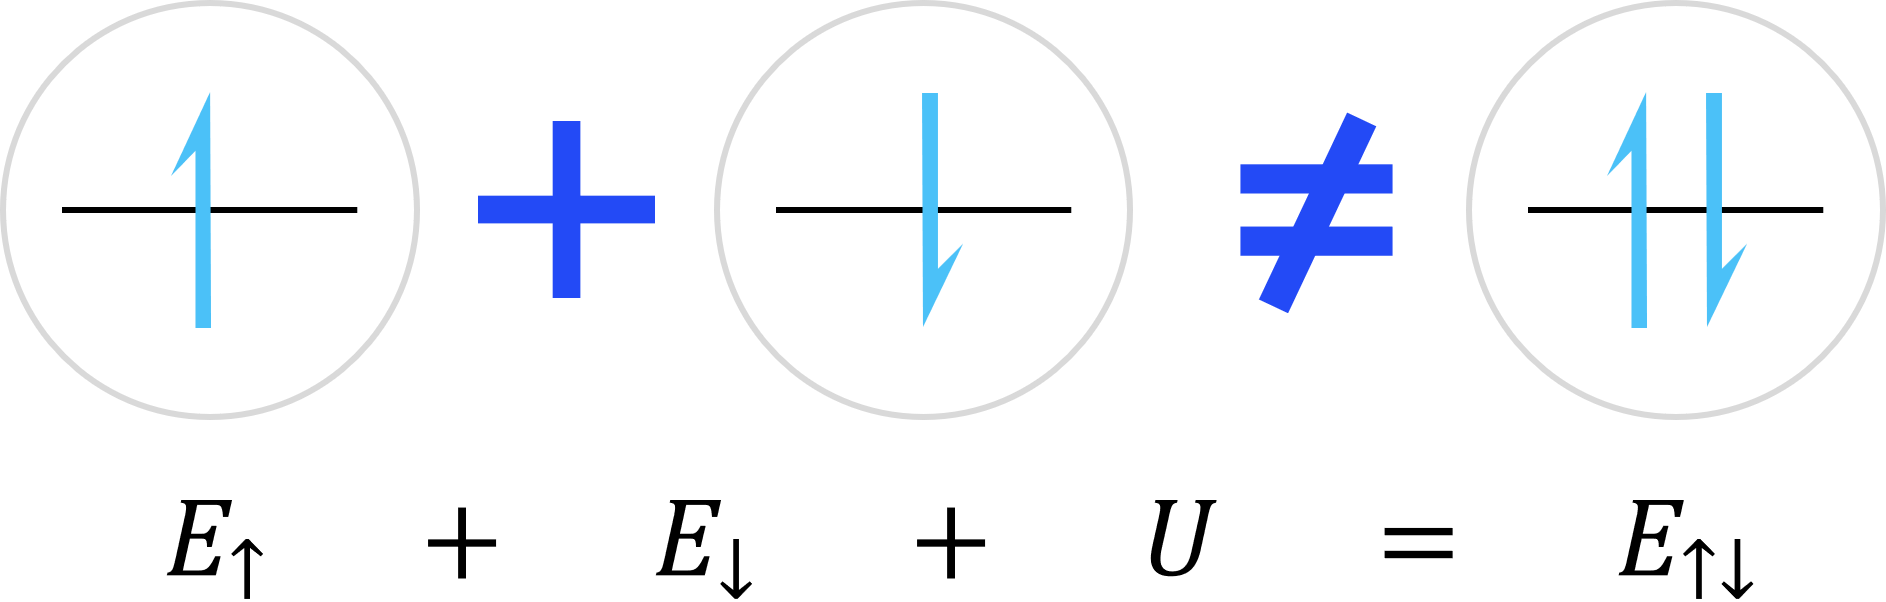
\includegraphics[height=0.72in,width=2.42in,viewport=0 0 1430 460,clip]{Figures/correalation-energy.png}
\caption{\tiny \textrm{The meaning of $U$, when the Coulomb-interaction of each electron is taken into account.}}%(与文献\cite{EPJB33-47_2003}图1对比)
\label{Tetrahedron_weight}
\end{figure}
}

\frame
{
\frametitle{$U$值的物理含义}
根据\textrm{Hubbard}模型,\textrm{$U$}值定义为两个原子间转移一个$d$\,电子的能量,即\upcite{PRB44-943_1991}
$$2(d^n)\rightarrow d^{n+1}+d^{n-1}$$
因此有
$$U=E(d^{n+1})+E(d^{n-1})-2E(d^n)$$
\textrm{L(S)DA}是弱耦合的平均场(\textrm{mean-filed, MF})理论,对$d$、$f$\,能带\textcolor{blue}{含有自旋和轨道简并体系},引入\textrm{Hubbard}参数$U$
\begin{displaymath}
	H_I=\frac12U\sum\limits_{\nu,\nu^{\prime}\atop(\nu\neq\nu^{\prime})}n_{i\nu}n_{i\nu^{\prime}}
\end{displaymath}
其中$\nu=(m,\sigma)$,因此\textrm{LDA}基础上\textcolor{red}{考虑自旋和轨道极化能量校正}
\begin{displaymath}
	\begin{aligned}
		E=E_{\mathrm{LDA}}+&\frac12\sum_{m,m^{\prime},\sigma}U(n_{m,\sigma}-n_0)(n_{m^{\prime},-\sigma}-n_0)\\
		+&\frac12\sum_{m\neq m^{\prime},\sigma}(U-J)(n_{m,\sigma}-n_0)(n_{m^{\prime},\sigma}-n_0)
	\end{aligned}
\end{displaymath}
}

\frame
{
	\frametitle{$U$值的物理含义}
	单电子势也因此与轨道相关
	\begin{displaymath}
		\begin{aligned}
			V_{m,\sigma}=V_{\mathrm{LDA}}+&\sum_{m^{\prime}}U(n_{m^{\prime},-\sigma}-n_0)\\
			+&\sum_{m\neq m^{\prime}}(U-J)(n_{m^{\prime},\sigma}-n_0)
		\end{aligned}
	\end{displaymath}
\begin{figure}[h!]
\centering
\vspace*{-0.25in}
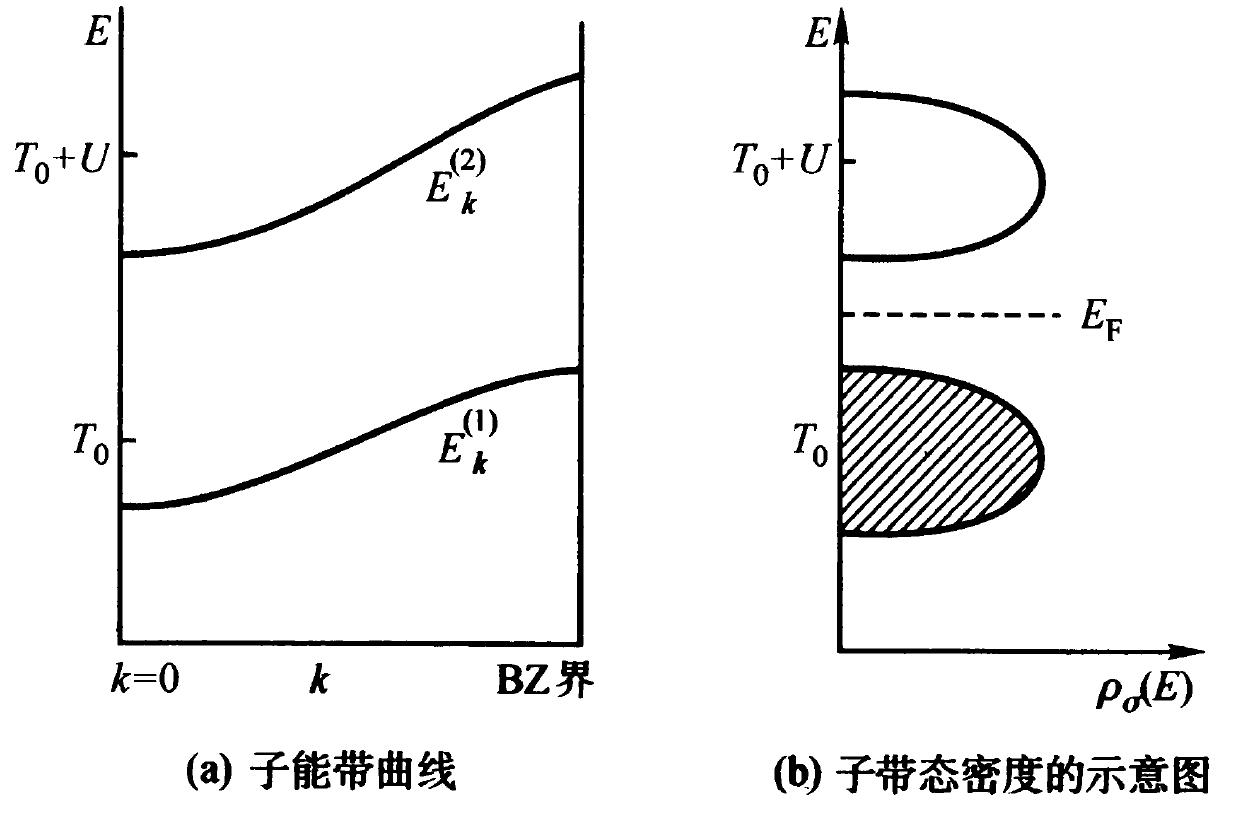
\includegraphics[height=2.0in,width=3.1in,viewport=0 0 1250 880,clip]{Figures/LDA_U-4.png}
\caption{\tiny \textrm{The schematic band structure (a) and DOS (b) of systems including localized electrons calculated based on LDA.}}%(与文献\cite{EPJB33-47_2003}图1对比)
\label{LDA_U-4}
\end{figure}
}

\subsection{自相互作用校正}
\frame
{
	\frametitle{自相互作用校正}
	上述$+U$校正方案是平均场近似下局域电子均匀占据模型得到的,\textcolor{blue}{根据\textrm{Anderson~}杂质模型,可有自能校正方案}
	\begin{itemize}
		\item 价电子中离域电子$s$、$p$电子只用轨道无关的\textrm{L(S)DA}单粒子势函数描述
		\item 在\textrm{LDA}近似下,当体系中含有$d$电子离子,$d$-$d$电子相互作用对\textrm{Coulomb~}能的贡献由$d$~电子数$N$确定\\$UN(N-1)/2$
		\item 将价电子中的局域电子$d$、$f$~电子划分为子体系,这些电子间的\textrm{Coulomb}~相互作用用轨道相关的模型\textrm{Hamiltonian}描述\\$\frac12U\sum\limits_{i\neq j}n_in_j$
	\end{itemize}
	考虑\textrm{Hubbard}校正后,总能量泛函可表示为\upcite{PRB48-16929_1993}
	$$E=E_{\mathrm{LDA}}-\frac{UN(N-1)}2+\frac12U\sum\limits_{i\neq j}n_in_j$$
}

\frame
{
	\frametitle{自相互作用校正}
	\begin{itemize}
		\item 在自相互作用模型下,轨道能量
	$$\varepsilon_i=\partial E/\partial n_i=\varepsilon_{\mathrm{LDA}}+U(\frac12-n_i)$$
	\textcolor{blue}{考虑轨道极化后}
		\item 对于\textcolor{blue}{占据轨道}($n_i=1$),局域轨道\textcolor{blue}{能量被移动$-\frac U2$}
		\item 对于\textcolor{red}{未占据轨道}($n_i=0$),局域轨道\textcolor{red}{能量被移动$\frac U2$}
		\item 轨道相关的单电子势函数
			$$V_i(\vec r)=V_{\mathrm{LDA}}(\vec r)+U(\frac12-n_i)$$
			\textcolor{orange}{这样构造的单电子势满足精确密度泛函的跳跃不连续要求}
	\end{itemize}
}

\frame
{
	\frametitle{自相互作用校正}
	以上讨论中忽略了电子交换作用和$d$-$d$电子\textrm{Coulomb}相互作用的非球形部分贡献
	\begin{itemize}
		\item 考虑电子交换的贡献后
			\begin{displaymath}
				\begin{aligned}
					E=&\frac12U\sum_{m,m^{\prime},\sigma}n_{m,\sigma}n_{m^{\prime},-\sigma}\\
					+&\frac12(U-J)\sum_{m,m^{\prime},\sigma\atop(m\neq m^{\prime})}n_{m,\sigma}n_{m^{\prime},\sigma}
				\end{aligned}
			\end{displaymath}
	在\textrm{LDA}中,考虑电子交换时要求满足$(N_{\uparrow}=N_{\downarrow},N=N_{\uparrow}+N_{\downarrow})$,因此$d$-$d$\,电子\textrm{Coulomb}相互作用可以表示为
	$$UN(N-1)/2-JN(N-2)/4$$
	\end{itemize}
}

\frame
{
	\frametitle{自相互作用校正}
	\begin{itemize}
		\item 考虑非球形部分对\textrm{Coulomb}和交换作用的影响
			\begin{displaymath}
				\begin{aligned}
					&U_{mm^{\prime}}=\sum_ka_kF^k\\
					&J_{mm^{\prime}}=\sum_kb_kF^k\\
					&a_k=\frac{4\pi}{2k+1}\sum_{q=-k}^k\langle lm|Y_{kq}|lm\rangle\langle lm|Y_{kq}^{\ast}|lm^{\prime}\rangle\\
					&b_k=\frac{4\pi}{2k+1}\sum_{q=-k}^k|\langle lm|Y_{kq}|lm^{\prime}\rangle|^2
				\end{aligned}
			\end{displaymath}
	这里$F^k$是\textrm{Slater}积分,$\langle lm|Y_{kq}|lm^{\prime}\rangle$是三个球谐函数积分
	\end{itemize}
	\textcolor{red}{注意:~}\textcolor{blue}{以上讨论忽略了形如$\langle mm^{\prime}|\frac1{r_{12}}|m^{\prime\prime}m^{\prime\prime\prime}\rangle$的\textrm{Coulomb}和交换矩阵的非对角元部分(原子多组态理论)贡献}
}

\frame
{
	\frametitle{自相互作用校正}
	最后得到自相互作用校正的总能量泛函
	\begin{displaymath}
		\begin{aligned}
			\textcolor{blue}{E}=\textcolor{red}{E_{\mathrm{LDA}}}+&\big[UN(N-1)/2-JN(N-2)/4\big]\\
			+&\frac12\sum_{m,m^{\prime},\sigma}U_{mm^{\prime}}n_{m,\sigma}n_{m^{\prime},-\sigma}\\
			+&\frac12\sum_{m,m^{\prime},\sigma\atop(m\neq m^{\prime})}(U_{mm^{\prime}}-J_{mm^{\prime}})n_{m,\sigma}n_{m^{\prime},\sigma}
		\end{aligned}
	\end{displaymath}
	单电子势
	\begin{displaymath}
		\begin{aligned}
			V_{m,\sigma}(\vec r)=V_{\mathrm{LDA}}(\vec r)+&\sum_{m^{\prime}}(U_{mm^{\prime}}-U+\frac12J)n_{m,-\sigma}\\
			+&\sum_{m^{\prime}\neq m}(U_{mm^{\prime}}-J_{mm^{\prime}}-U+\frac12J)n_{m,\sigma}\\
			+&(U-\frac12J)(\frac12-n_{m,\sigma})-\frac14J
		\end{aligned}
	\end{displaymath}
}

\frame
{
	\frametitle{自相互作用校正}
	根据\textrm{Clebsch-Gordan (CG)}系数的性质,可以确定参数$U$和$J$与\textrm{Slater}积分$F^k$(对$d$\,电子需要计算$F^0$、$F^2$、$F^4$)的关系
	\begin{displaymath}
		\begin{aligned}
			U=&\frac1{(2l+1)^2}\sum_{mm^{\prime}}U_{mm^{\prime}}=F^0\\
			U-J=&\frac1{2l(2l+1)}\sum_{mm^{\prime}}(U_{mm^{\prime}}-J_{mm^{\prime}})\\
			=&F^0-(F^2+F^4)	\\
			J=&(F^2+F^4)/14
		\end{aligned}
	\end{displaymath}
	由参数$U$和$J$确定\textrm{Slater}积分,只需要确定$F^4/F^2$的比值,一般地,$F^4/F^2$的比值在$0.62\sim0.63$,如果将$F^4/F^2$确定为0.625,因此有
	\begin{displaymath}
		\begin{aligned}
			F^2=&\frac{14}{1.625}J\\
			F^4=&0.625F^2
		\end{aligned}
	\end{displaymath}
}

\subsection{\rm{Rotationally invariant LDA+}$U$}
\frame
{
	\frametitle{\textrm{Rotationally invariant LDA+}$U$}
	上述\textrm{LDA}+$U$计算对基函数的选择依赖很显著,只适用于简单体系,更一般的做法是用密度矩阵$n_{mm^{\prime}}^{\sigma}$代替电荷占据数$n_{m\sigma}$,这称为\textrm{Rotationally invariant LDA}+$U$\upcite{PRB52-R5467_1995}

局域电子的密度矩阵定义为
\begin{displaymath}
	n_{mm^{\prime}}^{\sigma}=-\frac1{\pi}\int^{\mathrm{E_F}}\Im G_{ilm,ilm^{\prime}}^{\sigma}(E)\mathrm{d}E
\end{displaymath}
其中$G_{ilm,ilm^{\prime}}^{\sigma}=\langle ilm\sigma|(E-H)^{-1}|ilm^{\prime}\sigma\rangle$,是局域表示中的\textrm{Green's function}的矩阵元,$H$是有效单电子\textrm{Hamltonian}

用密度矩阵$\{n\}$表示的一般\textrm{LDA+}$U$的总能量泛函表示为
\begin{displaymath}
	\begin{aligned}
		E^{\mathrm{LDA}+U}[\rho^{\sigma}(\vec r),\{n^{\sigma}\}]=&E^{\mathrm{LSDA}}[\rho^{\sigma}(\vec r)]+E^U[\{n^{\sigma}\}]\\
		-&E_{\mathrm{dc}}[\{n^{\sigma}\}]
	\end{aligned}
\end{displaymath}
其中$\rho^{\sigma}(\vec r)$是自旋为$\sigma$电子密度,$E^{\mathrm{LDA}}[\rho^{\sigma}(\vec r)]$是\textrm{LSDA}的泛函表达式
}

\frame
{
	\frametitle{\textrm{Rotationally invariant LDA+}$U$}
	根据平均场理论
	\begin{displaymath}
		\begin{aligned}
			E^U[\{n\}]=&\frac12\sum_{\{m\},\sigma}\{\langle m,m^{\prime\prime}|V_{ee}|m^{\prime},m^{\prime\prime\prime}\rangle n_{mm^{\prime}}^{\sigma}n_{m^{\prime\prime}m^{\prime\prime\prime}}^{-\sigma}\\
			+&(\langle m,m^{\prime\prime}|V_{ee}|m^{\prime},m^{\prime\prime\prime}\rangle\\
			-&\langle m,m^{\prime\prime}|V_{ee}|m^{\prime\prime\prime},m^{\prime}\rangle)n_{mm^{\prime}}^{\sigma}n_{m^{\prime\prime}m^{\prime\prime\prime}}^{\sigma}\}
		\end{aligned}
	\end{displaymath}
	这里$V_{ee}$是$nl$电子间的屏蔽\textrm{Coulomb}相互作用
\begin{displaymath}
	\begin{aligned}
		E_{\mathrm{dc}}[\{n^{\sigma}\}]=\frac12Un(n-1)-\frac12[(U-J)n^{\uparrow}(n^{\uparrow}-1)+Un^{\downarrow}(n^{\downarrow}-1)]
	\end{aligned}
\end{displaymath}
其中$n^{\sigma}=\mathrm{Tr}(n_{mm^{\prime}}^{\sigma})$并且$n=n^{\uparrow}+n^{\downarrow}$,$U$和$J$是屏蔽\textrm{Coulomb}和交换参数

\textcolor{red}{注意}:当密度矩阵退化为对角阵($n_{mm^{\prime}}^{\sigma}=n_m^{\sigma}\delta_{mm^{\prime}}$),\textrm{Rotationally invariant}就变成原始的\textrm{LDA}+$U$方案
}

\frame
{
	\frametitle{\textrm{Rotationally invariant LDA+}$U$}
	有效单电子势
	\begin{displaymath}
		\begin{aligned}
			V_{mm^{\prime}}^{\sigma}=&\sum_{m^{\prime\prime}m^{\prime\prime\prime}}\{\langle m,m^{\prime\prime}|V_{ee}|m^{\prime},m^{\prime\prime\prime}\rangle n_{m^{\prime\prime}m^{\prime\prime\prime}}^{-\sigma}\\
			+&(\langle m,m^{\prime\prime}|V_{ee}|m^{\prime},m^{\prime\prime\prime}\rangle\\
			-&\langle m,m^{\prime\prime}|V_{ee}|m^{\prime\prime\prime},m^{\prime}\rangle)n_{m^{\prime\prime}m^{\prime\prime\prime}}^{\sigma}\}\\
			-&U(n-\frac12)+J(n^{\sigma}-\frac12)
		\end{aligned}
	\end{displaymath}
	\begin{itemize}
		\item \textcolor{blue}{$V_{ee}$的确定}:只考虑\textrm{LSDA}近似下原子的有效电子-电子相互作用球形部分的贡献
%		\item \textcolor{blue}{矩阵元$n_{mm^{\prime}}^{\sigma}$也是局域的,\textrm{LSDA}能量本征值对密度矩阵的二次变分即相互作用能}:
	\end{itemize}
	类似地,上述矩阵元可以用有效\textrm{Slater}积分表示
	\begin{displaymath}
		\langle m,m^{\prime\prime}|V_{ee}|m^{\prime},m^{\prime\prime\prime}\rangle=\sum_ka_k(m,m^{\prime},m^{\prime\prime},m^{\prime\prime\prime})F^k
	\end{displaymath}
	这里$0\leqslant k\leqslant 2l$
}

\frame
{
	\begin{displaymath}
		\begin{aligned}
			a_k(m,m^{\prime},m^{\prime\prime},m^{\prime\prime\prime})=&\frac{4\pi}{2k+1}\sum_{q=-k}^k\langle lm|Y_{kq}|lm^{\prime}\rangle\\
			&\times\langle lm^{\prime\prime}|Y_{kq}^{\ast}|lm^{\prime\prime\prime}\rangle
		\end{aligned}
	\end{displaymath}
	当$|lm^{\prime}\rangle$的基函数是球谐函数,可有
	\begin{displaymath}
		\begin{aligned}
			a_k(m,m^{\prime},m^{\prime\prime},m^{\prime\prime\prime})=&\sum_{q=-k}^k(2l+1)^2(-1)^{m+q+m^{\prime}}\\
			&\times\left(
			\begin{matrix}
				l &k &l\\
				0 &0 &0
			\end{matrix}
			\right)^2\left(
			\begin{matrix}
				l &k &l\\
				-m &q &m^{\prime}
			\end{matrix}\right)\\
			&\times\left(
			\begin{matrix}
				l &k &l\\
				-m^{\prime\prime} &-q &m^{\prime\prime\prime}
			\end{matrix}\right)
		\end{aligned}
	\end{displaymath}
类似地,对$d$\,电子只需要$F^0$、$F^2$、$F^4$\\一般仍取$U=F^0$,$J=(F^2+F^4)/14$,$F^4/F^2\sim 0.625$
}

\frame
{
	\frametitle{\textrm{Simplified Rotationally invariant LDA+}$U$}
	\textrm{L(S)DA}+$U$建立了\textrm{DFT-LSDA}和非约束\textrm{Hartree-Fock(UHF)}的关联\upcite{PRB57-1505_1998},采用模型\textrm{Hamiltonian}
\begin{displaymath}
	\hat H=\frac{\bar U}2\sum_{m,m^{\prime},\sigma}\hat n_{m,\sigma}\hat n_{m^{\prime},-\sigma}+\frac{(\bar U-\bar J)}2\sum_{m\neq m^{\prime},\sigma}\hat n_{m,\sigma}\hat n_{m^{\prime},\sigma}
\end{displaymath}
这里$\hat n_{\sigma}$是在位占据粒子数算符,其期望值为$n_{\sigma}$,$\bar U$和$\bar J$是屏蔽\textrm{Coulomb}和电子交换相互作用矩阵元的球形平均,因此能量泛函可表示为
	\begin{displaymath}
		\begin{aligned}
			E_{\textrm{LSDA+}U}=&E_{\textrm{LSDA}}+\frac{(\bar U-\bar J)}2\sum_{\sigma}\left[\mathrm{Tr}\rho^{\sigma}-\mathrm{Tr}(\rho^{\sigma}\rho^{\sigma})\right]\\
			=&E_{\textrm{LSDA}}+\frac{(\bar U-\bar J)}2\sum_{\sigma}\left[\left(\sum_j\rho_{jj}^{\sigma}\right)-\left(\sum_{j,l}\rho_{jl}^{\sigma}\rho_{lj}^{\sigma}\right)\right]
		\end{aligned}
	\end{displaymath}
	其中$\rho_{jl}^{\sigma}$是$d$\,电子密度矩阵,对每个离子密度矩阵是对角化,其本征值为$n_{m,\sigma}$
}

\frame
{
	\frametitle{\textrm{Simplified Rotationally invariant LDA+}$U$}
	类似地,单电子势矩阵元可定义为
	\begin{displaymath}
		V_{jl}^{\sigma}\equiv\frac{\delta E_{\mathrm{LDA+}U}}{\rho_{lj}^{\sigma}}=\frac{\delta E_{\mathrm{LDA}}}{\delta \rho_{lj}^{\sigma}}+(\bar U-\bar J)\left[\frac12\delta_{jl}-\rho_{jl}^{\sigma}\right]
	\end{displaymath}
	当总能量用\textrm{Kohn-Sham}本征值$\{\varepsilon_j\}$表示
	\begin{displaymath}
		E_{\textrm{LSDA+}U}=\textcolor{blue}{E_{\textrm{LSDA}}[\textcolor{red}{\{\varepsilon_j\}}]}+\frac{(\bar U-\bar J)}2\sum_{l,j,\sigma}\rho_{lj}^{\sigma}\rho_{jl}^{\sigma}
	\end{displaymath}
	这里最后一项对应的是\textrm{double-counting}校正
}
%\frame
%{
%\frametitle{LDA+$U$近似处理含$d$、$f$\,电子的重元素体系}
%对局域的$d$\,或$f$\,电子,用含\textrm{$U$}的模型\textrm{Hamiltonian}考虑$d$-$d$或$f$-$f$间相互作用(定域\textrm{Coulomb}相互作用\textrm{$U$})。%,离域的\textit{s}\,和\textit{p}\,电子的运动用\textrm{LDA}近似描述。
%\begin{itemize}
%\setlength{\itemsep}{10pt}
%	\item \textrm{LDA+$U$}方法最重要的特征:通过参数\textrm{$U$}校正\textrm{LDA}中的电子自相互作用,使单电子能量变化出现不连续。%计算表明LDA+U方法对含有定域强Coulomb相互作用的体系是有效的\upcite{PRB48-16929_1993,JPCS56-1521_1995,EPL36-551_1996}。无论
%	\item \textrm{LDA+$U$}方法是平均场近似,对含有近似芯层的局域4$f$\,电子的镧系元素离子还是过渡金属的氧化物(金属的3$d$\,电子与氧原子2$p$\,电子有很强的相互作用)体系都有效。如\textrm{FeSi}和\textrm{LaCaO$_3$}等体系,\textrm{LDA+$U$}能给出有关于金属-绝缘体转变的有用信息。甚至用于含有5$f$\,电子的化合物的研究也取得一定的成功。
%\end{itemize}
%}
%------------------------------------------------------------------------Reference----------------------------------------------------------------------------------------------
		\frame[allowframebreaks]
{
\begin{thebibliography}{99}
\frametitle{主要参考文献}
{\tiny
	\bibitem{PRL49-1691_1982}\textrm{P. Perdew, R. G. Parr, M. Levy and J. L. Balduz, Jr., \textit{Phys. Rev. Lett.} \textbf{49} (1982), 1691}
	\bibitem{PRB44-943_1991}\textrm{V. I. Anisimov, J. Zaanen and O.K. Andersen. \textit{Phys. Rev.} B, \textbf{44} (1991), 943}
	\bibitem{PRB48-16929_1993}\textrm{V.I. Anisimov, I.V. Solovyev, M.A. Korotin, M.T. Czyzyk and G.A. Sawatzky. \textit{Phys. Rev.} B, \textbf{48} (1993), 16929}
	\bibitem{PRB52-R5467_1995}\textrm{A. I. Liechtenstein, V. I. Anisimov and J. Zaanen., \textit{Phys. Rev.} B, \textbf{52} (1995), R5467}
	\bibitem{PRB57-1505_1998}\textrm{S. L. Dudarev, G. A. Botton, S. Y. Savrasov, C. J. Humphreys and A. P. Sutton., \textit{Phys. Rev.} B, \textbf{57} (1998), 1505}
}
\end{thebibliography}
\nocite*{}
}
%-----------------------------------------------------------------------------------------------------------------------------------------------------------------------%
